\begin{savequote}[45mm]
\ascii{Any fool can write code that a computer can understand. Good programmers write code that humans can understand.}
\qauthor{\ascii{- Martin Flower}}
\end{savequote}

\chapter{系统架构} 
\label{ch:architecture}

\begin{content}

本章将阐述\tf{}的系统架构,并一个简单的例子,讲述图结构的变换过程;最后,通过挖掘会话管理的工作机制,加深理解\tf{}运行时的工作机理。

\end{content}

\section{系统架构}
	
\begin{content}

\tf{}的系统结构以\emph{\ascii{C API}}为界,\footnote{事实上,后端系统中也存在\ascii{Client}的代码,并常称它为前端系统在后端系统实现中的代理\ascii{Client}。在后面的章节,将详细地讨论这个问题。}将整个系统分为\emph{前端}和\emph{后端}两个子系统:

\begin{enum}
  \eitem{前端系统:提供编程模型,负责构造计算图;}
  \eitem{后端系统:提供运行时环境,负责执行计算图。} 
\end{enum}

\begin{figure}[!htbp]
\centering
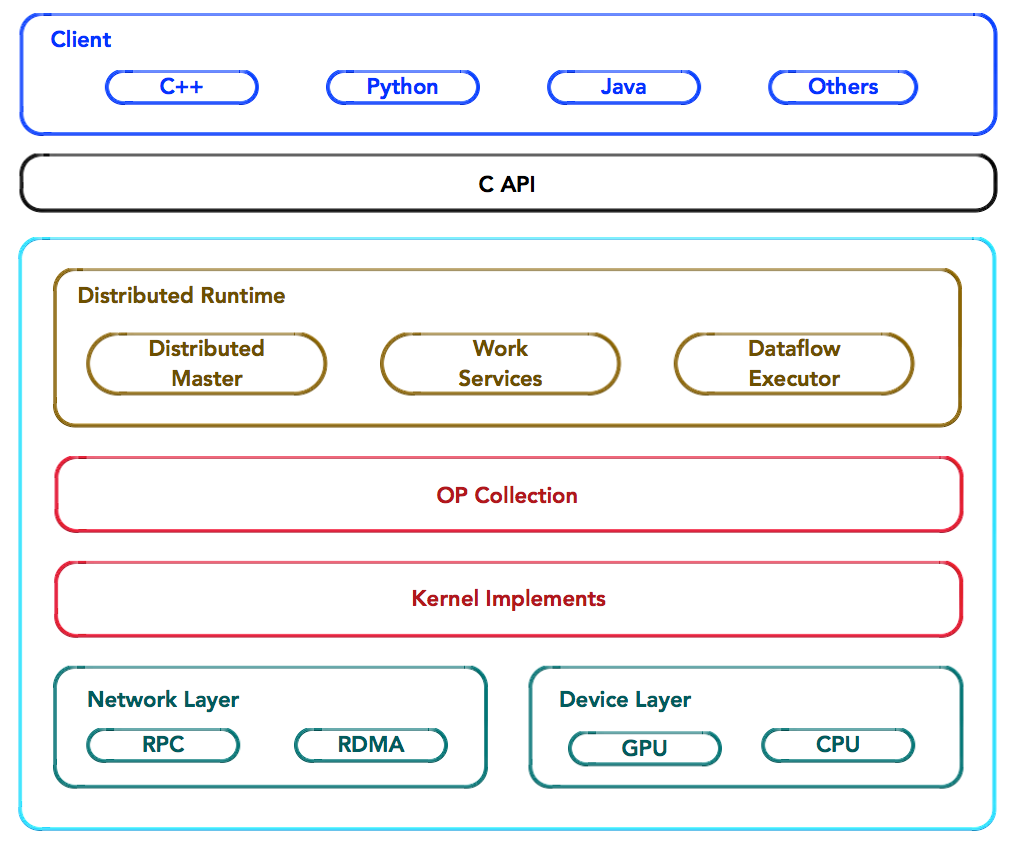
\includegraphics[width=0.9\textwidth]{figures/tf-architecture.png}
\caption{TensorFlow系统架构}
 \label{fig:tf-architecture}
\end{figure}

如\refig{tf-architecture}所示,重点关注系统中如下\ascii{4}个基本组件,它们是系统分布式运行时的核心。

\subsection{Client}

\ascii{Client}是前端系统的主要组成部分,它是一个支持多语言的编程环境。\ascii{Client}基于\ascii{TensorFlow}的编程接口,构造计算图。

目前,\ascii{TensorFlow}支持\ascii{Python}和\ascii{C++}的编程接口较为完善,尤其对\ascii{Python}的\ascii{API}支持最为全面。并且,对其他编程语言的\ascii{API}支持日益完善。

此时,\ascii{TensorFlow}并未执行任何的图计算,直至与后台计算引擎建立\ascii{Session},并以\ascii{Session}为桥梁,建立\ascii{Client}与\ascii{Master}之间的通道,将\ascii{Protobuf}格式的\ascii{GraphDef}序列化后发送至\ascii{Master},启动计算图的执行过程。

\subsection{Master}

在分布式的运行时环境中,\ascii{Client}根据\code{Session.run}传递整个计算图给后端的\ascii{Master};此时,计算图是完整的,常称为\emph{\ascii{Full Graph}}。

随后,\ascii{Master}根据\ascii{Client}通过\code{Session.run}传递\code{fetches}参数列表,反向遍历\ascii{Full Graph},并按照依赖关系,对其实施剪枝,最终计算得到最小的依赖子图,常称为\ascii{Client Graph}。

随后,\ascii{Master}负责将\ascii{Client Graph}按照任务的名称分裂\ascii{(split-by-task)}为多个子图片段,常称为\ascii{(Graph Partition)};其中,每个\ascii{Worker}对应一个\ascii{Graph Partition}。

随后,\ascii{Master}将\ascii{Graph Partition}分别注册到相应的\ascii{Worker}上,以便在不同的\ascii{Worker}上并发执行这些子图片段。

最后,\ascii{Master}将通知所有\ascii{Work}启动相应子图片段的执行;其中,\ascii{Work}之间可能存在数据交互,\ascii{Master}不参与两者之间的数据交换,它们两两互相通信,独立地完成交换数据,直至完成所有计算。

\subsection{Worker}

对于每一个任务,\tf{}都将启动一个\ascii{Worker}实例。\ascii{Worker}主要负责如下\ascii{3}个方面的职责:

\begin{enum}
  \eitem{处理来自\ascii{Master}的请求;}
  \eitem{按照拓扑排序算法执行本地子图,并调度\ascii{OP}的\ascii{Kernel}实现;} 
  \eitem{协同任务之间的数据通信。}
\end{enum}

首先,\ascii{Worker}收到\ascii{Master}发送过来的图执行命令,此时的计算图相对于\ascii{Worker}是完整的,也称为\ascii{Full Graph},它对应于\ascii{Master}的一个\ascii{Graph Partition}。随后,\ascii{Worker}也会执行图剪枝,得到最小依赖的\ascii{Client Graph}。

随后,\ascii{Worker}根据当前可用的硬件环境,包括\ascii{(GPU/CPU)}资源,按照\ascii{OP}设备的约束规范,再将\ascii{Client Graph}分裂\ascii{(split-by-device)}为多个\ascii{Graph Partition};其中,每个计算设备对应一个\ascii{Graph Partition};随后,\ascii{Worker}启动所有的\ascii{Graph Partition}的执行。

最后,对于每一个计算设备,\ascii{Worker}将按照计算图中节点之间的依赖关系执行拓扑排序算法,并依次调用\ascii{OP}的\ascii{Kernel}实现,完成\ascii{OP}的运算(一种典型的多态实现技术)。其中,\ascii{Worker}还要负责将\ascii{OP}运算的结果发送到其他的\ascii{Worker}上去;或者接受来自其他\ascii{Worker}发送给它的运算结果,以便实现\ascii{Worker}之间的数据交互。

\subsection{Kernel}

\ascii{Kernel}是\ascii{OP}在某种硬件设备的特定实现,它负责执行\ascii{OP}的具体运算。目前,\ascii{TensorFlow}系统中包含\ascii{200}多个标准的\ascii{OP},包括数值计算,多维数组操作,控制流,状态管理等。

一般每一个\ascii{OP}根据设备类型都会存在一个优化了的\ascii{Kernel}实现。在运行时,运行时根据\ascii{OP}的设备约束规范,及其本地设备的类型,为\ascii{OP}选择特定的\ascii{Kernel}实现,完成该\ascii{OP}的计算。

其中,大多数\ascii{Kernel}基于\code{Eigen::Tensor}实现。\code{Eigen::Tensor}是一个使用\ascii{C++}模板技术,为多核\ascii{CPU/GPU}生成高效的并发代码。但是,\ascii{TensorFlow}也可以灵活地直接使用\ascii{cuDNN}实现更高效的\ascii{Kernel}。

此外,\ascii{TensorFlow}实现了矢量化技术,在高吞吐量、以数据为中心的应用需求中,及其移动设备中,实现更高效的推理。如果对于复合\ascii{OP}的子计算过程很难表示,或执行效率低下,\ascii{TensorFlow}甚至支持更高效的\ascii{Kernel}注册,其扩展性表现非常优越。

\end{content}

\section{图控制}

\begin{content}

通过一个最简单的例子,进一步抽丝剥茧,逐渐挖掘出\tf{}计算图的控制与运行机制。

\subsection{组建集群}

如\refig{tf-1ps-1worker}所示。假如存在一个简单的分布式环境:\ascii{1 PS + 1 Worker},并将其划分为两个任务:

\begin{enum}
  \eitem{\ascii{ps0}: 使用\code{/job:ps/task:0}标记,负责模型参数的存储和更新;}
  \eitem{\ascii{worker0}: \code{/job:worker/task:0}标记,负责模型的训练。} 
\end{enum}

\begin{figure}[!htbp]
\centering
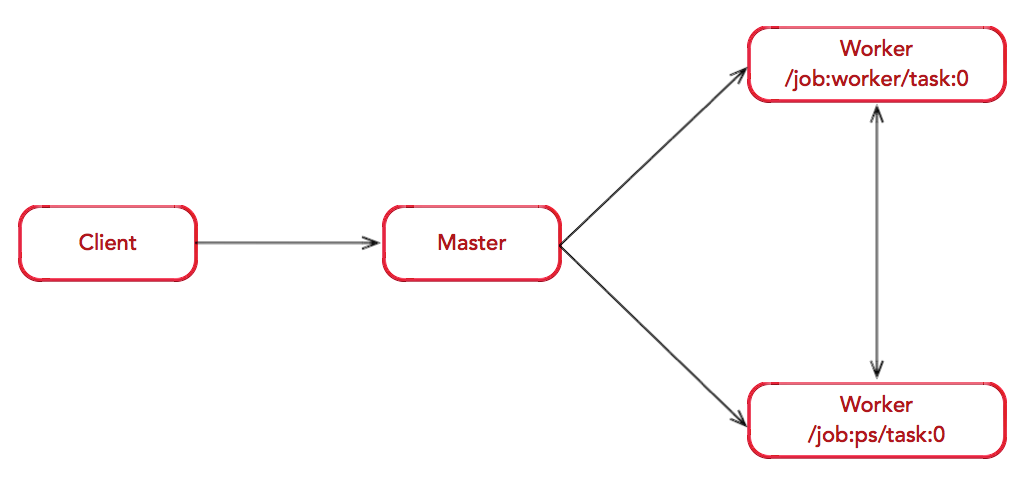
\includegraphics[width=0.9\textwidth]{figures/tf-1ps-1worker.png}
\caption{TensorFlow集群:\ascii{1 PS + 1 Worker}}
 \label{fig:tf-1ps-1worker}
\end{figure}

\subsection{图构造}

如\refig{tf-graph-construction}所示。\ascii{Client}构建了一个简单计算图;首先,将$w$与$x$进行矩阵相乘,再与截距$b$按位相加,最后更新至$s$中。

\begin{figure}[!htbp]
\centering
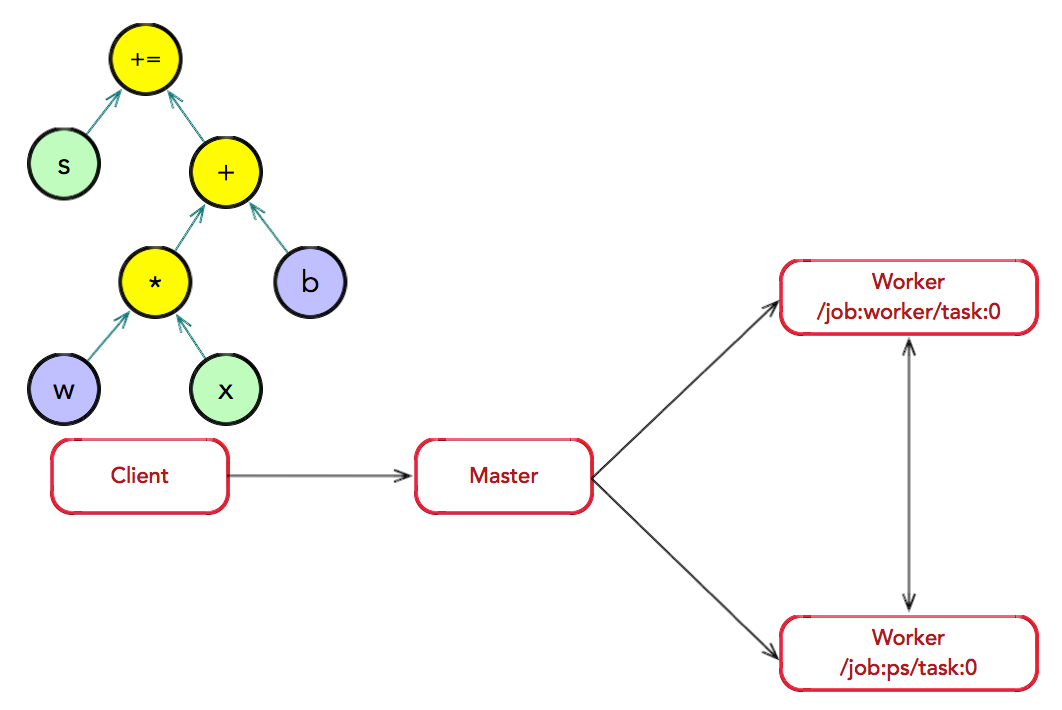
\includegraphics[width=0.9\textwidth]{figures/tf-graph-construction.png}
\caption{图构造}}
 \label{fig:tf-graph-construction}
\end{figure}

\subsection{图执行}

如\refig{tf-graph-execution}所示。首先,\ascii{Client}创建一个\code{Session}实例,建立与\ascii{Master}之间的通道;接着,\ascii{Client}通过调用\code{Session.run}将计算图传递给\ascii{Master}。

随后,\ascii{Master}便开始启动一次\ascii{Step}的图计算过程。在执行之前,\ascii{Master}会实施一系列优化技术,例如\emph{公共表达式消除},\emph{常量折叠}等。最后,\ascii{Master}负责任务之间的协同,执行优化后的计算图。

\begin{figure}[!htbp]
\centering
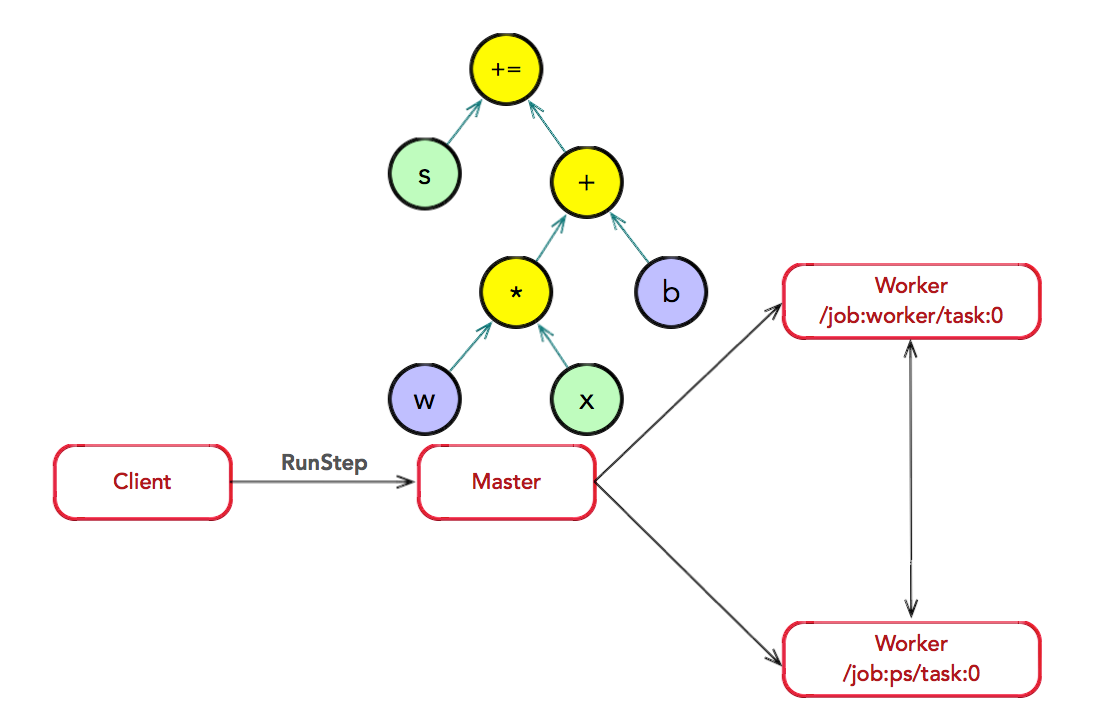
\includegraphics[width=0.9\textwidth]{figures/tf-graph-execution.png}
\caption{图执行}}
 \label{fig:tf-graph-execution}
\end{figure}

\subsubsection{图分裂}

如\refig{tf-graph-split-by-task}所示,存在一种合理的图划分算法。\ascii{Master}将模型参数相关的\ascii{OP}划分为一组,并放置在\ascii{ps0}任务上;其他\ascii{OP}划分为另外一组,放置在\ascii{worker0}任务上执行。

\begin{figure}[!htbp]
\centering
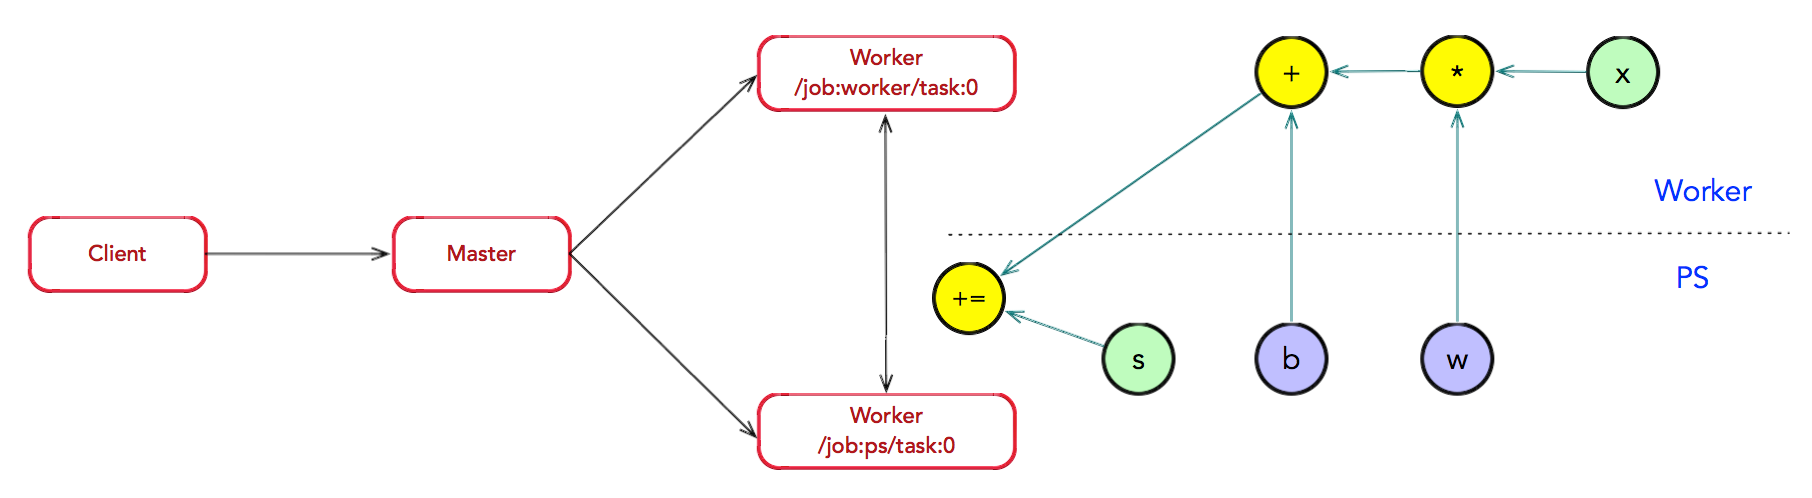
\includegraphics[width=1.0\textwidth]{figures/tf-graph-split-by-task.png}
\caption{图分裂:按任务划分}}
 \label{fig:tf-graph-split-by-task}
\end{figure}

\subsubsection{子图注册}

如\refig{tf-register-graph}所示。在图分裂过程中,如果计算图的边跨越节点或设备,\ascii{Master}将该边实施分裂,在两个节点或设备之间插入\ascii{Send}和\ascii{Recv}节点,实现数据的传递。

其中,\code{Send}和\code{Recv}节点也是\ascii{OP},只不过它们是两个特殊的\ascii{OP},由内部运行时管理和控制,对用户不可见;并且,它们仅用于数据的通信,并没有任何数据计算的逻辑。

最后,\ascii{Master}通过调用\code{RegisterGraph}接口,将子图注册给相应的\ascii{Worker}上,并由相应的\ascii{Worker}负责执行运算。

\begin{figure}[!htbp]
\centering
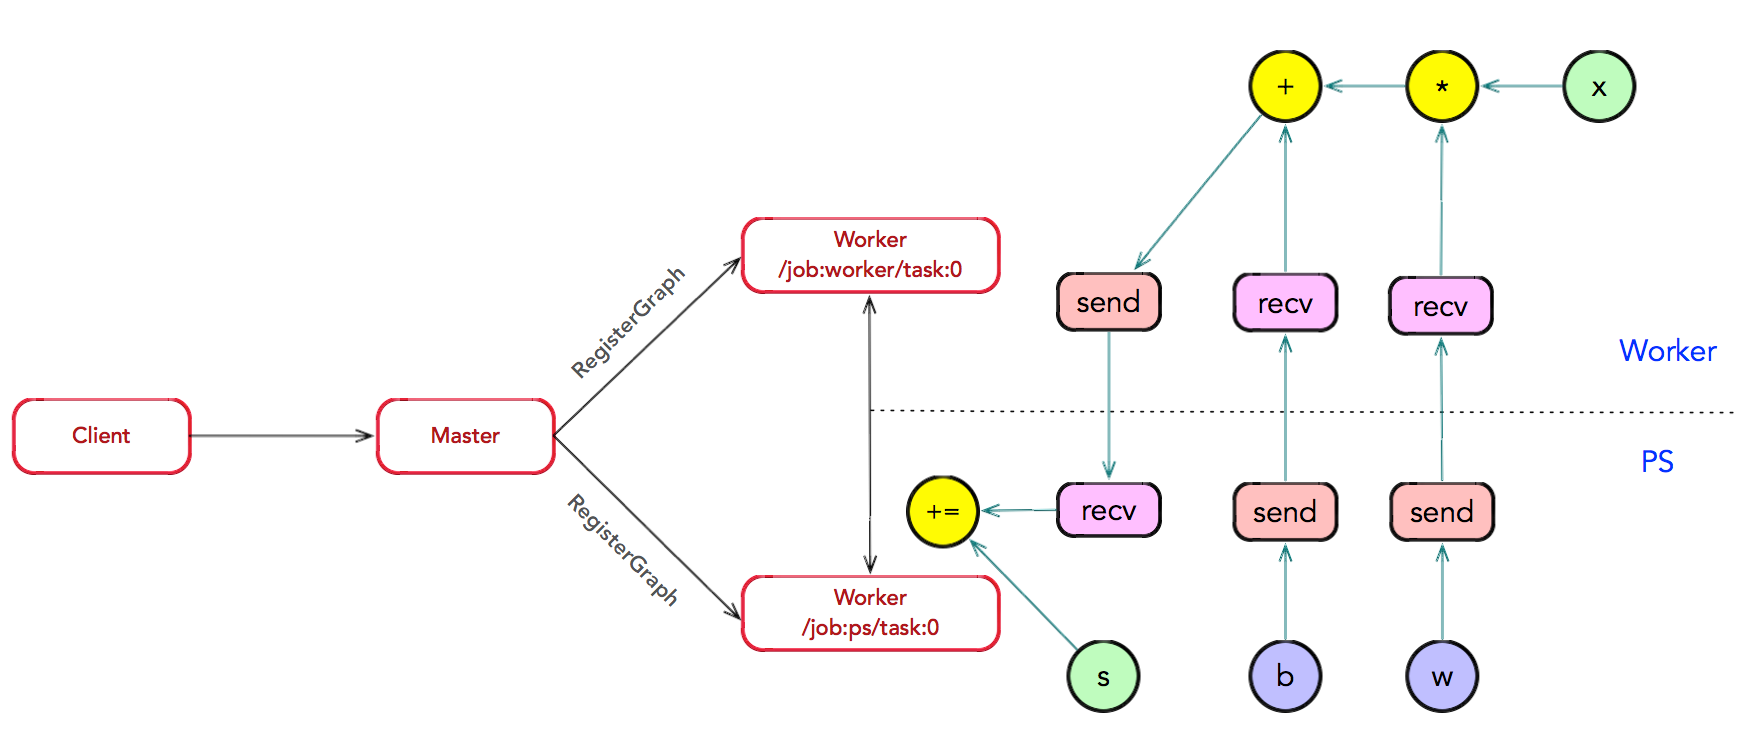
\includegraphics[width=1.0\textwidth]{figures/tf-register-graph.png}
\caption{子图注册:插入Send和Recv节点}}
 \label{fig:tf-register-graph}
\end{figure}

\subsubsection{子图运算}

如\refig{tf-run-graph}所示。\ascii{Master}通过调用\code{RunGraph}接口,通知所有\ascii{Worker}执行子图运算。其中,\ascii{Worker}之间可以通过调用\code{RecvTensor}接口,完成数据的交换。

\begin{figure}[!htbp]
\centering
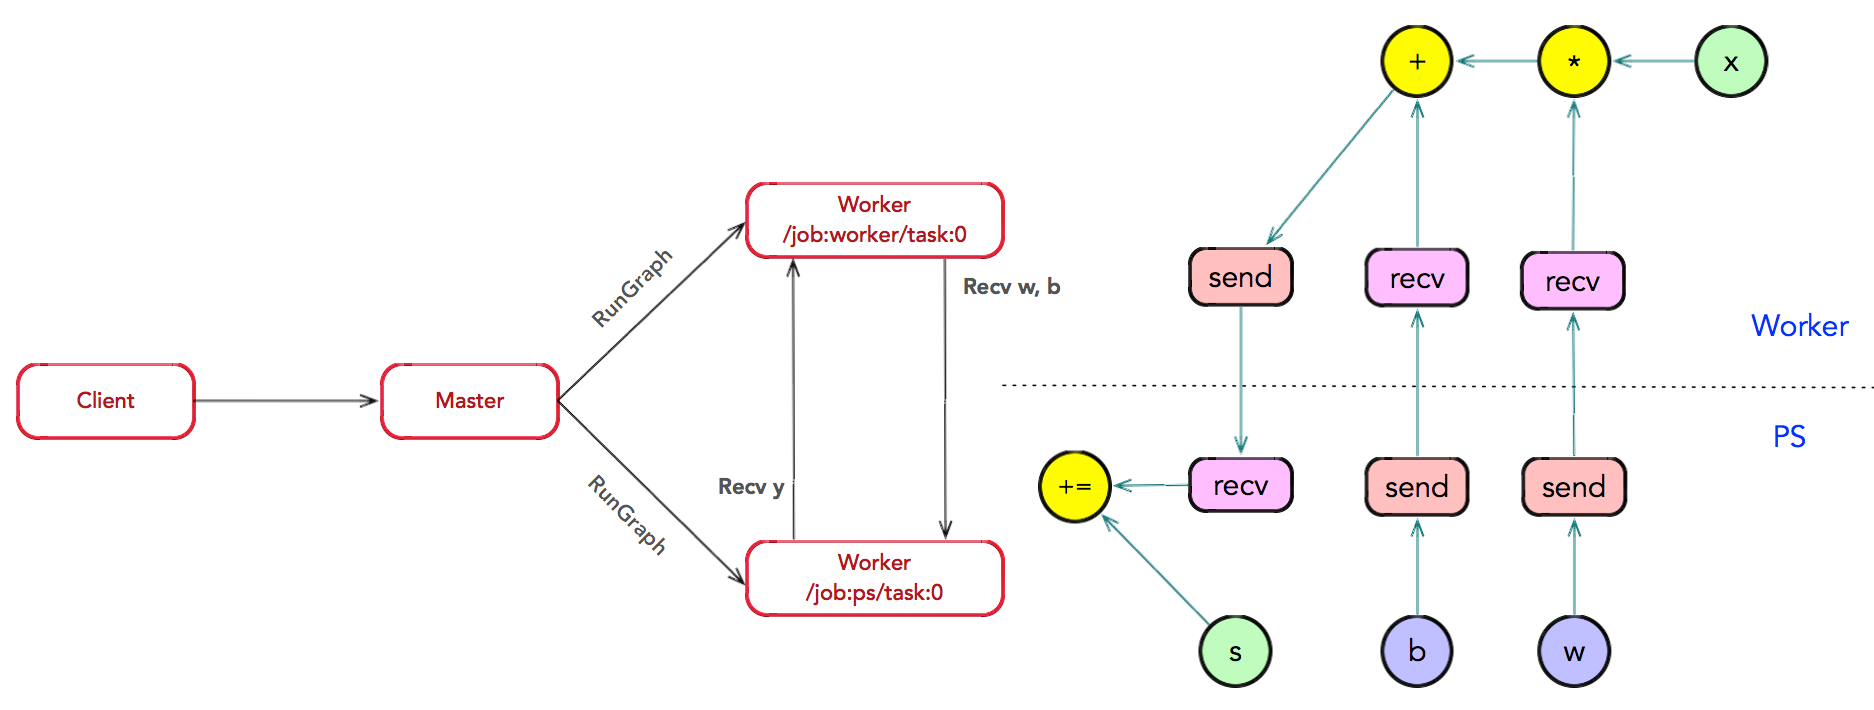
\includegraphics[width=1.0\textwidth]{figures/tf-run-graph.png}
\caption{子图执行}}
 \label{fig:tf-run-graph}
\end{figure}

\end{content}

\section{会话管理}
	
\begin{content}

接下来,通过概述会话的整个生命周期过程,及其与图控制之间的关联关系,进一步揭开运行时的内部运行机制。

\subsection{创建会话}

首先,\ascii{Client}\emph{首次}执行\code{tf.Session.run}时,会将整个图序列化后,通过\ascii{GRPC}发送\code{CreateSessionRequest}消息,将图传递给\ascii{Master}。

随后,\ascii{Master}创建一个\code{MasterSession}实例,并用全局唯一的\code{handle}标识,最终通过\code{CreateSessionResponse}返回给\ascii{Client}。如\refig{tf-create-session-overview}所示。

\begin{figure}[!h]
\centering
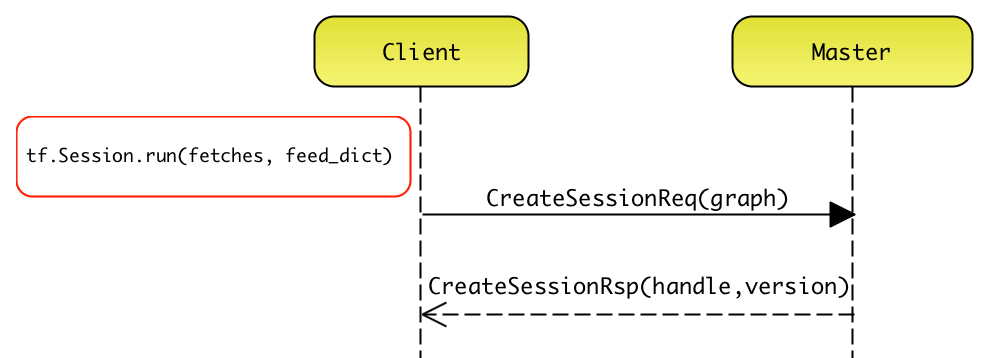
\includegraphics[width=0.9\textwidth]{figures/tf-create-session-overview.png}
\caption{创建会话}}
 \label{fig:tf-create-session-overview}
\end{figure}

\subsection{迭代运行}

随后,\ascii{Client}会启动迭代执行的过程,并且称每次迭代为一次\ascii{Step}。此时,\ascii{Client}发送\code{RunStepRequest}消息给\ascii{Master};并且消息携带\code{handle}标识,用于\ascii{Master}索引相应的\code{MasterSession}实例。如\refig{tf-run-step-overview}所示。

\begin{figure}[!h]
\centering
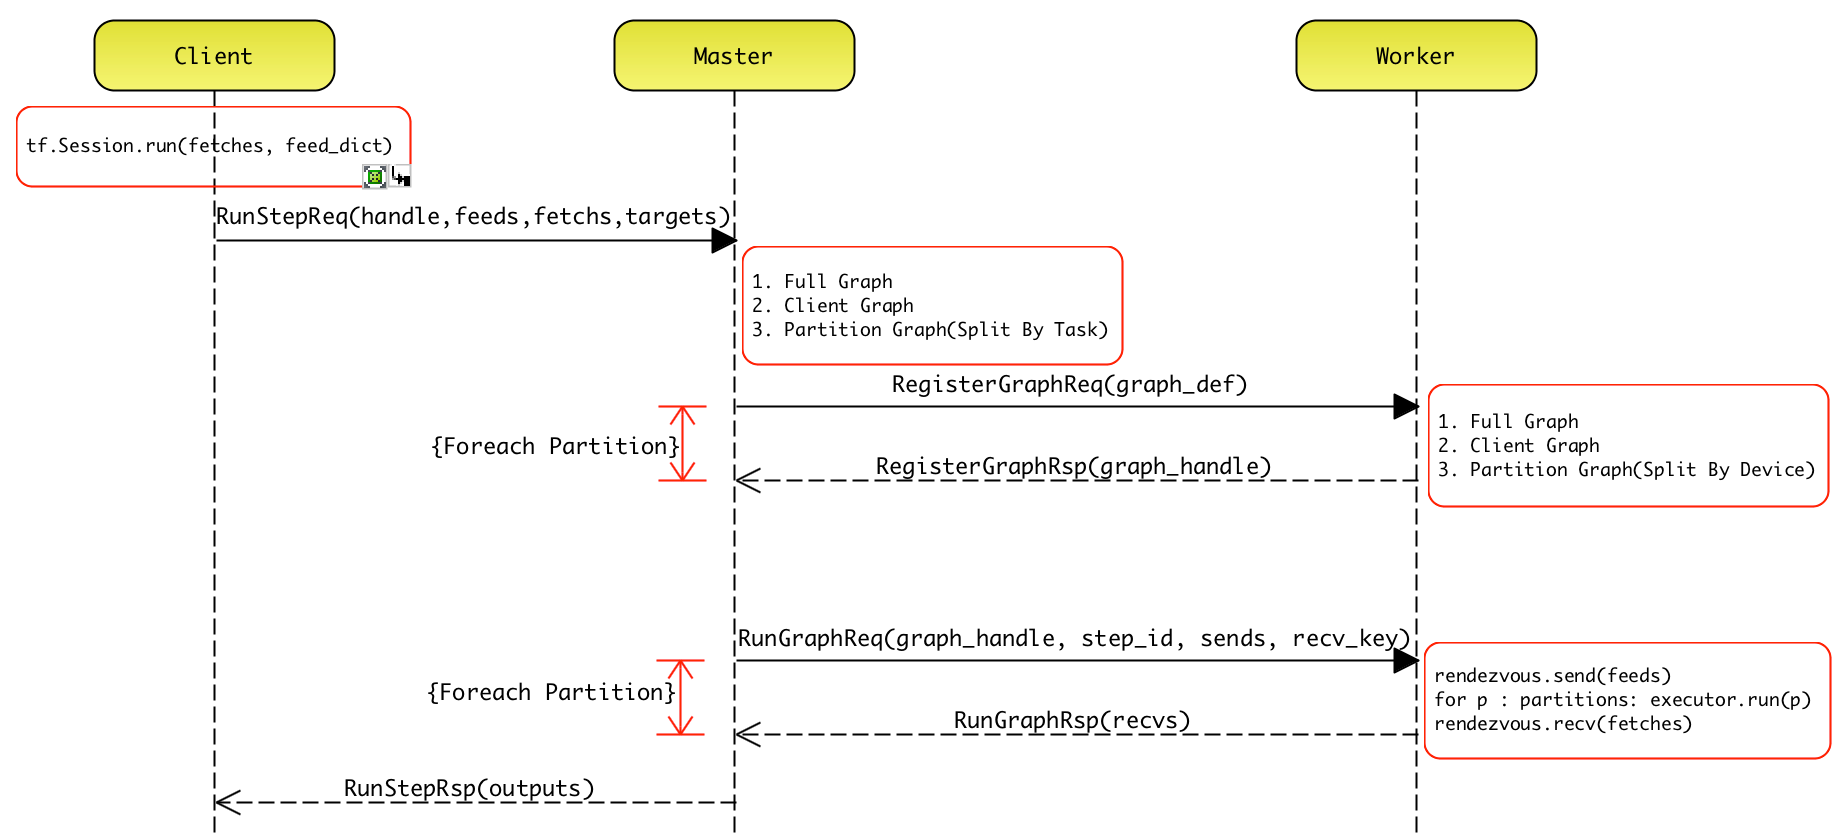
\includegraphics[width=1.0\textwidth]{figures/tf-run-step-overview.png}
\caption{迭代执行}}
 \label{fig:tf-run-step-overview}
\end{figure}

\subsubsection{注册子图}

\ascii{Master}收到\code{RunStepRequest}消息后,将执行图剪枝,分裂,优化等操作;最终按照任务\ascii{(Task)},将图划分为多个子图片段\ascii{(Graph Partition)}。

随后,\ascii{Master}向各个\ascii{Worker}发送\code{RegisterGraphRequest}消息,将子图片段依次注册到各个\ascii{Worker}节点上。

当\ascii{Worker}收到\code{RegisterGraphRequest}消息后,再次执行图剪枝,分裂操作;最终按照设备\ascii{(Device)},将图划分为多个子图片段\ascii{(Graph Partition)}。\footnote{在分布式运行时,图分裂经过两级分裂过程。在\ascii{Master}上按照任务分裂,而在\ascii{Worker}按照设备分裂;因此得到结果都称为子图片段,它们仅存在范围,及其大小的差异。}

当\ascii{Worker}完成子图注册后,通过返回\code{RegisterGraphReponse}消息,并携带\code{graph\_handle}标识。这是因为\ascii{Worker}可以并发注册并运行多个子图,每个子图使用\code{graph\_handle}唯一标识。

\subsubsection{运行子图}

\ascii{Master}完成子图注册后,将广播所有\ascii{Worker}并发执行所有子图。这个过程是通过\ascii{Master}发送\code{RunGraphRequest}消息给\ascii{Worker}完成的;其中,消息中携带\code{graph\_handle}标识,用于\ascii{Worker}索引相应的子图。

\ascii{Worker}收到消息\code{RunGraphRequest}消息后,按照如下形式化了的算法执行子图的运算。

\begin{leftbar}
  \begin{python}
def run_graph(feeds):
  rendezvous.send(feeds)
  for p in partitions: 
    executor.run(p)
  rendezvous.recv(fetches)
  \end{python}
\end{leftbar}

首先,\ascii{Worker}根据\code{graph\_handle}索引相应的子图;然后,并发执行所包含的所有子图片段。其中,每个子图片段放置在单独的\code{Executor}中执行,\code{Executor}将按照拓扑排序算法完成子图片段的计算。

\subsubsection{交换数据}

如果两个设备之间需要交换数据,则通过插入\ascii{Send/Recv}节点完成的。特殊地,如果两个\ascii{Worker}之间需要交换数据,则需要涉及跨主机,或跨进程的通信。

此时,需要通过接收端主动发送\code{RecvTensorRequest}消息到发送方,再从发送方的信箱里取出对应的\ascii{Tensor},并通过\code{RecvTensorResponse}返回。如\refig{tf-recv-tensor-overview}所示。


\begin{figure}[!h]
\centering
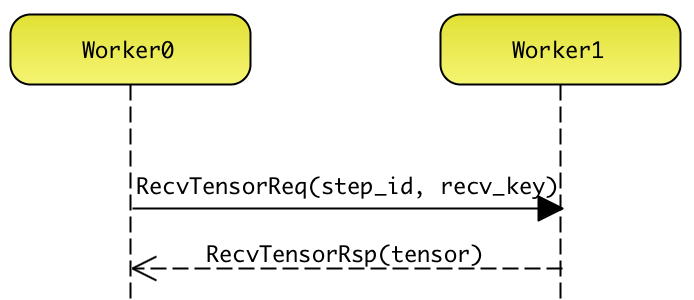
\includegraphics[width=0.7\textwidth]{figures/tf-recv-tensor-overview.png}
\caption{Worker之间的数据交换}}
 \label{fig:tf-recv-tensor-overview}
\end{figure}

\subsection{关闭会话}

经过许多次迭代执行后,\ascii{Client}向\ascii{Master}发送\code{CloseSessionReq}消息;\ascii{Master}收到消息后,开始释放\code{MasterSession}所持有的所有资源。如\refig{tf-close-session-overview}所示。

\begin{figure}[!h]
\centering
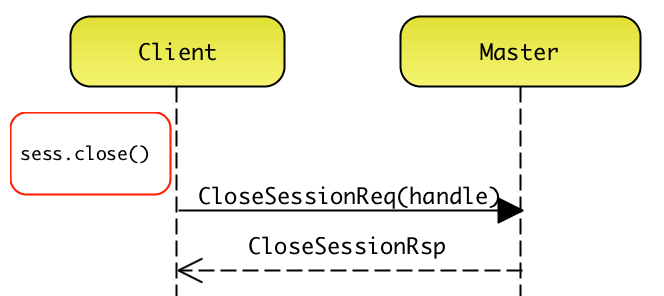
\includegraphics[width=0.7\textwidth]{figures/tf-close-session-overview.png}
\caption{关闭会话}}
 \label{fig:tf-close-session-overview}
\end{figure}

\end{content}
